\documentclass[12pt]{article}
\usepackage[margin=1in]{geometry} 
\usepackage{amsmath}
\usepackage{amssymb}
\usepackage{siunitx}
\usepackage{float}
\usepackage{tikz}
\def\checkmark{\tikz\fill[scale=0.4](0,.35) -- (.25,0) -- (1,.7) -- (.25,.15) -- cycle;} 
\usepackage{url}
\usepackage[siunitx,american,RPvoltages]{circuitikz}
\ctikzset{capacitors/scale=0.7}
\ctikzset{diodes/scale=0.7}
\usepackage{tabularx}
\newcolumntype{C}{>{\centering\arraybackslash}X}
\renewcommand\tabularxcolumn[1]{m{#1}}% for vertical centering text in X column
\usepackage{tabu}
\usepackage[spanish,es-tabla,activeacute]{babel}
\usepackage{babelbib}
\usepackage{booktabs}
\usepackage{pgfplots}
\usepackage{hyperref}
\hypersetup{colorlinks = true,
            linkcolor = black,
            urlcolor  = blue,
            citecolor = blue,
            anchorcolor = blue}
\usepgfplotslibrary{units, fillbetween} 
\pgfplotsset{compat=1.16}
\usepackage{bm}
\usetikzlibrary{arrows, arrows.meta, shapes, 3d, perspective, positioning,mindmap,trees,backgrounds}
\renewcommand{\sin}{\sen} %change from sin to sen
\usepackage{bohr}
\setbohr{distribution-method = quantum,insert-missing = true}
\usepackage{elements}
\usepackage{verbatim}
\usepackage[edges]{forest}
\usepackage{etoolbox}
\usepackage{schemata}
\usepackage{appendix}
\usepackage{listings}

\definecolor{color_mate}{RGB}{255,255,128}
\definecolor{color_plas}{RGB}{255,128,255}
\definecolor{color_text}{RGB}{128,255,255}
\definecolor{color_petr}{RGB}{255,192,192}
\definecolor{color_made}{RGB}{192,255,192}
\definecolor{color_meta}{RGB}{192,192,255}
\newcommand\diagram[2]{\schema{\schemabox{#1}}{\schemabox{#2}}}

\definecolor{codegreen}{rgb}{0,0.6,0}
\definecolor{codegray}{rgb}{0.5,0.5,0.5}
\definecolor{codepurple}{rgb}{0.58,0,0.82}
\definecolor{backcolour}{rgb}{0.95,0.95,0.92}

\lstdefinestyle{mystyle}{
    backgroundcolor=\color{backcolour},   
    commentstyle=\color{codegreen},
    keywordstyle=\color{magenta},
    numberstyle=\tiny\color{codegray},
    stringstyle=\color{codepurple},
    basicstyle=\ttfamily\footnotesize,
    breakatwhitespace=false,         
    breaklines=true,                 
    captionpos=b,                    
    keepspaces=true,                 
    numbers=left,                    
    numbersep=5pt,                  
    showspaces=false,                
    showstringspaces=false,
    showtabs=false,                  
    tabsize=2
}

\lstset{style=mystyle}
\usepackage{lastpage}
\usepackage{fancyhdr}
\pagestyle{fancy}
\setlength{\headheight}{42pt}
\setlength{\parindent}{0cm}
 
\begin{document}
\sisetup{unit-math-rm=\mathrm,math-rm=\mathrm} % change sinitx font
\sisetup{output-decimal-marker = {,}}
\lhead{Ingeniería en Mantenimiento Industrial \\ Escuela de Ingeniería Electromecánica \\ Tecnológico de Costa Rica} 
\rhead{Electricidad I \\ Tarea \#3  \\ Entrega: Semana 15} 
\cfoot{\thepage\ de \pageref{LastPage}}

A partir de los items del 8 al 15 del segundo examen parcial -cuyo enunciado puede encontrar \href{https://estudianteccr-my.sharepoint.com/:b:/g/personal/prof_juan_rojas_estudiantec_cr/Edpreo2lDBdFvutOSz8hA0gBmuoN-8wIpUa2Dnb22-bkQQ}{acá}- realice lo siguiente:
\begin{enumerate}
    \item Tomando en cuenta que los valores de $t_x$ van desde el 0.1 a 1 en incrementos de 0.1 y usando Python, Scilab, MATLAB cree un \emph{script} llamado ``respuetas'' que le permita realizar lo siguiente:
    \begin{itemize}
        \item calcular los valores de $A$, $B$, $C$, $D$, $E$, $F$, $G$, $H$ e $I$ para cada uno de los valores de $t_x$
        \item crear un archivo valores separados por comas (csv) que tenga en la primera columna tenga el nombre de las variables en el siguiente orden: 
        
        \begin{tabular}{cccccccccc}
            $t_x$& $A$& $B$& $C$& $D$& $E$& $F$& $G$& $H$
        \end{tabular}
        
        y luego en cada fila inferior las respuestas para cada valor de $t_x$ 
        \item generar una gráfica que en las abscisas tenga los valores del tiempo $t$ en segundos y en las ordenadas tenga el valor del voltaje $v_c(t)$ para cada valor de $t_x$
        \item generar una gráfica que en las abscisas tenga los valores del tiempo $t$ y en las ordenadas tenga el valor de la corriente $i_c(t)$ para cada valor de $t_x$
    \end{itemize}
    \item Realice un informe de su tarea llamado ``Informe\_t3.pdf'' usando \LaTeX. Incluya los cálculos y los datos finales de la tabla obtenida -en el archivo csv-, las gráficas solicitadas y algún texto complementario que permita al cliente entender lo que se realizó. Un machote se puede encontrar \href{https://www.overleaf.com/read/phnwtckqwqwc}{acá}
    \item Comprima todo en un solo archivo .zip y suba al TecDigital. Cualquier entrega tardía se califica con base en 70.
\end{enumerate}



Algunos tips:
\begin{itemize}
    \item Una forma sencilla de convertir un número en texto con un formato específico en Python es usar el operador de módulo. Ver mas \href{https://realpython.com/python-input-output/#the-string-modulo-operator}{acá}
    \item Las gráficas quedan mejor si se realizan juntas usando \href{https://matplotlib.org/3.1.1/api/_as_gen/matplotlib.pyplot.subplots.html}{subplot} 
    \item Cuando se requiere hacer varias gráficas en un solo eje simplemente se usa el comando \verb|plt.plot(...)| varias veces y luego de incluir todas las gráficas se usa el comando \verb|plt.show()|
\end{itemize}

Un ejemplo de como se pueden ver las gráficas -aunque en este caso son del ítem 2 al 7 del segundo examen parcial-:

\begin{figure}[H]
    \centering
    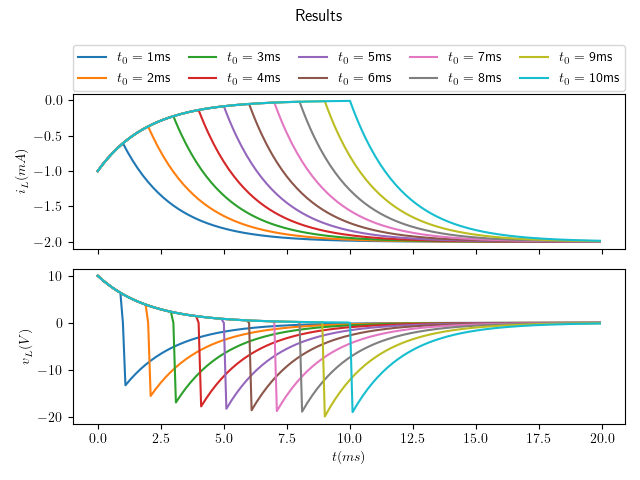
\includegraphics[width=0.9\linewidth]{fig/EP2_P1.png}
\end{figure}


% \bibliographystyle{IEEEtran}
% \bibliography{ref_tareas}

\end{document}